%!TEX root = paper.tex

\section{Wrapping Web Services}
\label{sec:wrapping_web_services}

Before third-party services can be used by our platform, they need to be provided with a service wrapper. In our approach, this is done in two steps: 
\begin{inparaenum}[(i)]
	\item constructing an exemplary service request, and 
	\item analysing the response received from the execution of the service, allowing the mapping of the response data to domain-specific concepts to be used as pre- and post-conditions.
\end{inparaenum}
From this input, the tool then generates the actual wrapper --- JavaScript code to be embedded into web gadgets.

\subsection{Constructing Service Requests} % (fold)
\label{sub:constructing_service_requests}

In this section we illustrate the interaction with RESTful services on simple GET requests\footnote{Other methods such as POST or SOAP-based services are also supported.}. 
In this case, a service request is assembled using its URL and a set of parameters. As an example, we will look at the eBay Shopping web service. 
To define the desired pre-condition and the type of post-condition of a new service wrapper, the service wrapper tool provides a form (not shown here). For the current example, we assume that the user has defined a pre-condition \emph{search\_key}.

We are invoking the service to retrieve a list of items corresponding to the search keyword ``USB'':

\begin{lstlisting}
http://open.api.sandbox.ebay.com/shopping?
  appid=KasselUn-efea-xxx&version=517&
  callname=FindItems&ItemSort=EndTime&
  QueryKeywords=USB&ResponseEncoding=XML
\end{lstlisting}

% The parameters used in the example are:
% \textbf{appid} (the application ID obtained to use the API),
% \textbf{version} (the API version),
% \textbf{callname} (in this case \emph{FindItems} to search through all items in eBay),
% \textbf{ItemSort} (sorting method for the list of items),
% \textbf{QueryKeywords} (list of keywords), and
% \textbf{ResponseEncoding} (format of the response message obtained by the invocation of the request).

% Note that we allow to edit example values for the input parameters, which can be used to test the service wrapper. 

% \begin{figure}
%   \begin{center} 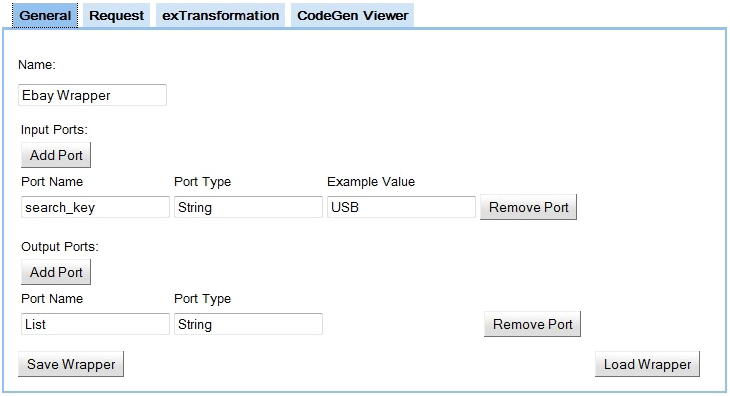
\includegraphics[width=\linewidth]{images/ServiceWrapperToolGVSWithPortDefinitions.png}
%     \caption{Configuring parameters of a service wrapper}
%     \label{fig:construct_pre_post_conditions}
%   \end{center}
% \end{figure}

% The service wrapper tool composes the request using a template string which will contain placeholders for input values. Before sending the request to the service, the placeholders are replaced with their corresponding values and the resulting URL is then ready to be sent as the service request.

The various parameters in the example are defined by the service provider. However, the most relevant one for our example is \emph{QueryKeywords}, which communicates to the services what we are looking for. 
An example of service request construction is shown in the Fig.~\ref{fig:construct_service_request}. In the ``Request'' input field the user enters an example HTTP request, e.g. the one above. The tool analyses the request and provides a form for editing the request parameters. In our example, the user has connected the service's \textit{QueryKeywords} parameter with the wrapper's \textit{search\_key} pre-condition. Requests constructed in this way can then be sent off to the service, whose response is shown in the bottom text area.

\begin{figure}
  \begin{center}
    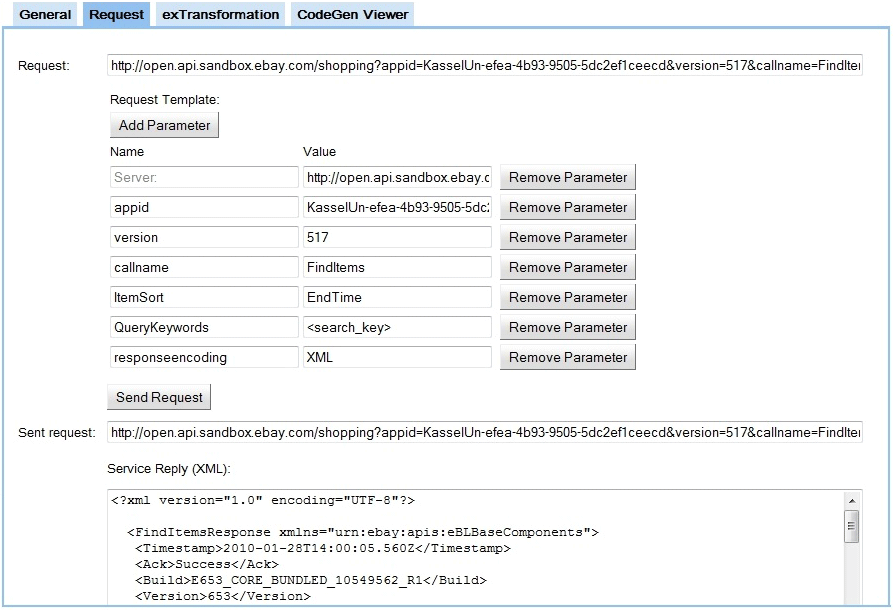
\includegraphics[width=\linewidth]{images/ServiceWrapperToolGVSWithRequestExample.png}
    \caption{Constructing the service request}
    \label{fig:construct_service_request}
  \end{center}
\end{figure}

% \subsubsection{Limitations} % (fold)
% \label{ssub:limitations}
% 
% It is worth pointing out that currently the wrapper tool is able to construct input ports for the wrappers using just basic types. To construct URL requests from more complex input parameters, as e.g. a person object, we are currently developing access operations that will allow to access the values of fields of complex objects. For example, the expression \emph{customer.address} may refer to the \emph{address} field of a \emph{customer} parameter.  
% 
% % subsubsection limitations (end)

% subsection constructing_service_requests (end)

\subsection{Interpreting Service Responses} % (fold)
\label{sub:interpreting_service_responses}

% A web service can choose to send a response message in any desired structured format. In our example, we assume an XML tree, but a JSON structure is equally possible.

% \subsubsection{Translation of the Response Tree into Facts} % (fold)
% \label{ssub:translation_xml_into_facts}

Once the service response has been retrieved, the transformation tab of the wrapper tool shows it as an interactive object tree, as seen in Fig.~\ref{fig:response_service_execution}. 

\begin{figure}
  \begin{center}
    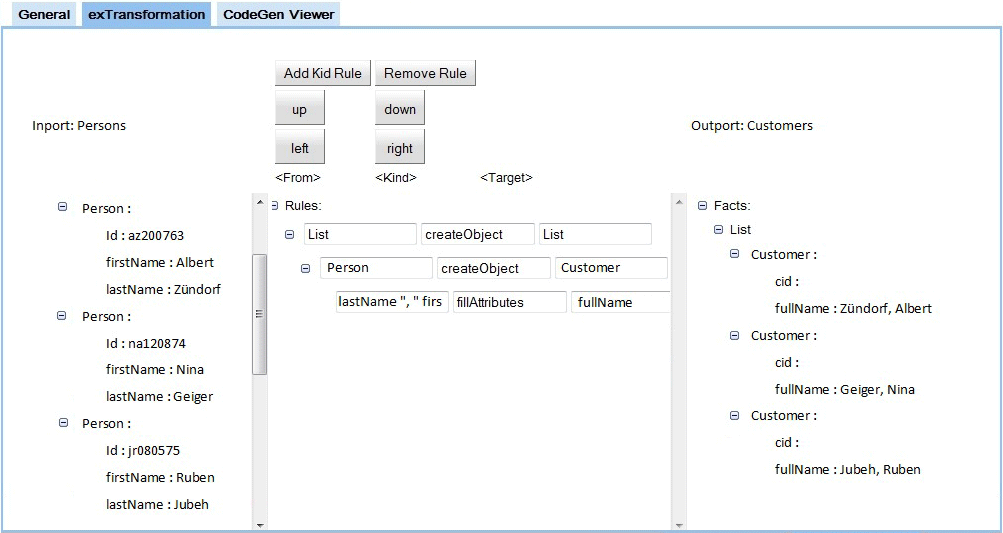
\includegraphics[width=\linewidth]{images/ServiceWrapperToolGVSWithTransformationRules.png}
    \caption{Rule-based transformation of service response}
    \label{fig:response_service_execution}
  \end{center}
\end{figure}

A transformation rule is used to analyse the response data and generate the wrapper's post-conditions. Such a rule is composed of three elements, as seen in the middle part of Fig.~\ref{fig:response_service_execution}. The \textit{from} field indicates the source elements to be translated by the rule. The second part defines the type of rule (see below). Thirdly, the target of the rule specifies a certain concept or attribute, to be created or filled. Rules can be chained together in a rule tree. A detailed explanation of the different rule types is as follows:

\paragraph{createObject} % (fold)
\label{par:createobject}

specifies the creation of a new post-condition of the type specified in the third part of the rule. In the example in Fig.~\ref{fig:construct_service_request}, the root rule could search for source elements with name \emph{FindItemsResponse} and create a post-condition of type \emph{List} for each such element. The resulting objects are shown in a facts tree in the right of the figure.

% paragraph createobject (end)

\paragraph{fillAttributes} % (fold)
\label{par:fillattributes}

only ever appear as sub-rules in the rule tree. They match source elements defined in the first part of the rule. The third part defines the attribute of the super-rule that will be filled (e.g., \emph{fullName} in Fig.~\ref{fig:response_service_execution}).
% In Fig.~\ref{fig:response_service_execution}, the third transformation rule matches elements with the name \emph{Title}. The 
% Note that this rule is a sub-rule of the second rule, which generates \emph{Product} objects. Thus, the sub-rule searches for \emph{Title} tags only in the subtree of the XML data that has been identified by an application of the parent rule before. For example, the \emph{Item} rule may just have been applied to the first \emph{Item} element of the XML data. Then, the \emph{Title} rule is applied only to the first \emph{Item} sub-tree of the XML data and thus it will find only one \emph{Title} element in that sub-tree (not visible in Figure ~\ref{fig:response_service_execution} ). The value of that \emph{Title} element is then transfered to the \emph{productName} attribute of the corresponding \emph{Product} object.

% paragraph fillattributes (end)

\paragraph{dummy} % (fold)
\label{par:dummy}

does not create or modify any objects but instead narrows the search space for their sub-rules, by selecting certain elements in the source tree and ignoring others.

% E.g., in Amazon product data, each item contains elements for \emph{minimum price}, \emph{maximum price}, and \emph{average price}. Each such element in turn contains a \emph{plain price} and \emph{formatted price}. In this case, a rule that searches for \emph{formatted price} elements within an \emph{Item} element would retrieve three matches. Using a dummy rule, we can first search for \emph{minimum price} elements and then search for \emph{formatted price} elements within that sub-tree.

% paragraph dummy (end)


Our tool follows an interactive paradigm. Any time a change to a transformation rule is done, the transformation process is triggered and the resulting facts tree is shown. This aids the user to deal with the complexity of the transformation rules, preventing errors or mistakes. In addition, the tool is ontology-driven, meaning that possible post-condition types and their attributes are selected from domain ontologies loaded in the system.
% therefore the service wrapper designer retrieves the domain-specific types from a backend server (such as the catalogue discussed in Section~\ref{sec:discovery}) together with the structure of each type, i.e. together with a description of the attributes of each object. Thus, the transformation rule editor is able to provide selection boxes for the target element of the rules. For a \emph{createObject} rule, this selection box shows the object types available for that domain. For the \emph{fillAttributes} rules, the selection box shows the attributes of the object type chosen in the parent rule. 
% In addition, we may provide some analysis tool, which will help to guarantee that the objects generated by the transformation rules conform to the object types defined in the corresponding conceptual model (see Section~\ref{ssec:ontology}). This helps to ensure that the objects generated by the designed service wrapper will be compatible for input parameters of subsequent filter steps and or gadgets.

% subsubsection translation_xml_into_facts (end)

% subsection interpreting_service_responses (end)

\subsection{Generating the Service Wrapper} % (fold)
\label{sub:generating_a_resource_adapter}

Once the wrapping of a service has been defined and tested in the tool, we generate an implementation of the desired specification in XML, HTML, and JavaScript, ready to be deployed and executed inside a web gadget. 

% subsection generating_a_resource_adapter (end)

% \subsection{Limitations} % (fold)
% \label{sub:limitations}
% 
% The rule driven approach presented above is somewhat limited. It is deliberately restricted to such a simple rule mechanism in order to keep things simple enough for end-users. Still, the selected approach suffices for many practical and real world cases. As a more complex example, the XML data for a person may provide two different tags for the first and the last name of a person. Contrarily, a person fact which conforms to a certain ontology for that domain may provide only one \emph{fullname} attribute that shall be filled by a concatenation of the first and the last name. To achieve this, the \textit{from} field of that transformation rule might look like: \texttt{lastname"', "`firstname}. We are also able to do some navigation in the XML tree to follow XRef elements. For example the attribute \texttt{grandmother} could be filled using \texttt{mother.mother} in the \textit{from} field. 
% 
% However, there are some transformations that these rules cannot perform. For example, we do not support any mathematical operations. Thus, transforming e.g. Fahrenheit into Celsius temperatures is not supported. To cover such  cases, intermediate object formats can be used which would allow generating objects to be further processed by additional filters. Such additional filters may be realised using (hand coded) operators, since some generic operators can act as filters for aggregation and conversions of objects from multiple sources. Then, service wrappers in combination with these filter operators will allow covering these complex cases.
% 
% subsection limitations (end)

% section restful_web_services_wrapper_tool (end)